\documentclass[12pt, a4paper]{article}
\usepackage{amsmath}
\usepackage{amsfonts}
\usepackage{amsthm}
\usepackage{mathtools}
\newtheorem{theorem}{Theorem}[section]
\newtheorem{definition}{Definition}[section]
\numberwithin{equation}{section}
\usepackage{pgfplots}
\pgfplotsset{width=10cm,compat=1.9}
\graphicspath{ {img/} }
\DeclareGraphicsExtensions{.png}

\title{word2vec}
\author{Kristian Wichmann}

\begin{document}
\maketitle

\section{A simple neural network}
Consider a feed forward neural network with one hidden layer, as shown in figure \ref{fig:nn}. The input layer consists of a row\footnote{Note that this is different from the column vector convention usually used.} vector $x$ of dimension $D_x$, i.e. $x\in\mathbb{R}^{1\times D_x}$. The hidden layer has $h$ neurons with a sigmoid activation function:
\begin{equation}
h=\sigma(xW^{(1)}+b^{(1)})=\sigma(z^{(1)}),\quad z^{(1)}=xW^{(1)}+b^{(1)}
\end{equation}
So $h\in\mathbb{R}^{1\times H}, W^{(1)}\in\mathbb{R}^{D_x\times H}, b^{(1)}\in\mathbb{R}^{1\times H}$. The output layer has $D_y$ softmax neurons:
\begin{equation}
\hat{y}=s(hW^{(2)}+b^{(2)})=s(z^{(2)}),\quad z^{(2)}=hW^{(2)}+b^{(2)}
\end{equation}
Similarly $\hat{y}\in\mathbb{R}^{1\times D_y}, W^{(2)}\in\mathbb{R}^{H\times D_y}, b^{(2)}\in\mathbb{R}^{1\times D_y}$.

\begin{figure}
\centering
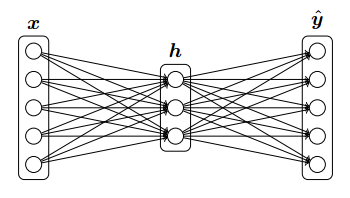
\includegraphics{w2v_nn}
\caption{The neural network.}
\label{fig:nn}
\end{figure}

\subsection{Error function}
Assuming a labelled dataset $x$ with the correct label $c$ encoded as a one-hot vector $t\in\mathbb{R}^{1\times D_y}$, so $t_i=\delta_{ic}$. We will use the cross-entropy error function:
\begin{equation}
J(x)=-\sum_{i=1}t_i\log\hat{y}_i
\end{equation}
Since $t$ is one-hot encoded, only the correct label $c$ will contribute to the sum, so:
\begin{equation}
J(x)=-\log\hat{y}_c
\end{equation}
This does not mean that the other components of $\hat{y}$ will not matter, since the softmax indirectly depends on all components.

\subsubsection{Derivative with respect to input}
We now wish to compute the derivative of $J(x)$ with respect to $x$. In shorthand, the chain rule gives us:
\begin{equation}
\frac{\partial J}{\partial x}=\frac{\partial J}{\partial\hat{y}}\frac{\partial \hat{y}}{\partial z^{(2)}}\frac{\partial z^{(2)}}{\partial h}\frac{\partial h}{\partial z^{(1)}}\frac{\partial z^{(1)}}{\partial x}
\end{equation}
Writing out indices explicitly:
\begin{equation}
\frac{\partial J}{\partial x_m}=\sum_{i=1}^{D_y}\sum_{j=1}^{D_y}\sum_{k=1}^H\sum_{l=1}^H\frac{\partial J}{\partial\hat{y}_i}\frac{\partial \hat{y}_i}{\partial z^{(2)}_j}\frac{\partial z^{(2)}_j}{\partial h_k}\frac{\partial h_k}{\partial z^{(1)}_l}\frac{\partial z^{(1)}_l}{\partial x_m}
\end{equation}
Let's compute these partial derivatives one by one:
\begin{equation}
\frac{\partial J}{\partial\hat{y}_i}=-\frac{\partial}{\partial\hat{y}_i}\log\hat{y}_c=-\frac{\delta_{ic}}{\hat{y}_c}
\end{equation}
The second is a standard result for the softmax function:
\begin{equation}
\frac{\partial \hat{y}_i}{\partial z^{(2)}_j}=s_i(z^{(2)})(\delta_{ij}-s_j(z^{(2)})=\hat{y}_i(\delta_{ij}-\hat{y}_j)
\end{equation}
Let's pause for a moment and combine the two:
\begin{equation}
\label{output_derivative}
\frac{\partial J}{\partial z^{(2)}_j}=\sum_{i=1}^{D_y}\frac{\partial J}{\partial\hat{y}_i}\frac{\partial \hat{y}_i}{\partial z^{(2)}_j}=-\sum_{i=1}^{D_y}\frac{\delta_{ic}}{\hat{y}_c}\hat{y}_i(\delta_{ij}-\hat{y}_j)
\end{equation}
The Kronecker delta removes the sum and we get:
\begin{equation}
-\frac{1}{\hat{y}_c}\hat{y}_c(\delta_{jc}-\hat{y}_j)=-(\delta_{jc}-\hat{y}_j)=\hat{y}_j-\delta_{jc}
\end{equation}
But $\delta_{jc}=t_j$, and we get that the derivative is simply equal to the \textit{error} in the output layer:
\begin{equation}
\label{ce_softmax}
\frac{\partial J}{\partial z^{(2)}_j}=\delta^{(2)}_j
\end{equation}
Here, $\delta^{(2)}_j=\hat{y}_j-\delta_{jc}$. Going back to the original derivation, the third derivative is:
\begin{equation}
\frac{\partial z^{(2)}_j}{\partial h_k}=W^{(2)}_{kj}
\end{equation}
The fourth uses a standard result for the sigmoid:
\begin{equation}
\frac{\partial h_k}{\partial z^{(1)}_l}=\delta_{kl}\sigma(z^{(1)}_l)(1-\sigma(z^{(1)}_l))=\delta_{kl}h_l(1-h_l)
\end{equation}
And finally:
\begin{equation}
\frac{\partial z^{(1)}_l}{\partial x_m}=W^{(1)}_{ml}
\end{equation}
Inserting, letting the delta functions cancel, and renaming indices, this becomes:
\begin{equation}
\label{error_derivative}
\frac{\partial J}{\partial x_i}=\sum_{j=1}^H\sum_{k=1}^{D_y}W^{(1)}_{ij}h_j(1-h_j)W^{(2)}_{jk}\delta^{(2)}_k
\end{equation}
We may rephrase this in terms of the backpropagated errors in the hidden layer:
\begin{equation}
\delta^{(1)}_j=\sum_{k=1}^{D_y}h_j(1-h_j)W^{(2)}_{jk}\delta^{(2)}_k
\end{equation}
Now equation \ref{error_derivative} can be rewritten as:
\begin{equation}
\frac{\partial J}{\partial x_i}=\sum_{j=1}^H\sum_{k=1}^{D_y}W^{(1)}_{ij}h_j(1-h_j)W^{(2)}_{jk}\delta^{(2)}_k=\sum_{j=1}^H W^{(1)}_{ij}\delta^{(1)}_j
\end{equation}

\section{The word2vec algorithm}

\subsection{The situation}
Imagine a large corpus of consecutive tokens (words) of length $T$. Each token comes from a vocabulary of size $W$. We wish to encode the tokens as vectors. To do this, we look at the words surrounding a given word in the corpus probabilistically. If $c$ is the center word, we can consider the probability of a word $j$ places away being $o$. We should really denote this probability $p_j(o|c)$, but for now we will simply call it $p(o|c)$.

\subsection{Softmax and word vectors}
If we have each word represented by vectors, an appropriate model for the probability could be a softmax over the entire vocabulary size:
\begin{equation}
p(o|c)=\frac{\exp(u_o^t v_c)}{\sum_{w=1}^W\exp(u_w^t v_c)}
\end{equation}
Note that each word $w$ has two vectors: $u_w$ and $v_w$. $u_w$ is for $w$ as an 'outside' word, and $v_w$ is for $w$ as a 'center' word.

\subsection{Error function and derivatives}
An appropriate error function for the softmax is the cross-entropy error. The situation is entirely analogous to the propagation from the hidden layer to the output layer in the neural network described in last section. I.e. it is described by equations \ref{output_derivative} and \ref{ce_softmax} with the following replacements:
\begin{itemize}
\item $j\mapsto o$
\item $z^{(2)}_j\mapsto z_o=u^t_o v_c$
\item $i\mapsto w$
\item $\hat{y}_i\mapsto p(o|c)$
\end{itemize}
So, the derivative with respect to $v_c$ is:
\begin{equation}
\label{v_derivative}
\frac{\partial J}{\partial v_c}=\sum_{o=1}^W\frac{\partial J}{\partial z_0}\frac{\partial z_0}{\partial v_c}=\sum_{o=1}^W\delta^{(2)}_o u_o=\sum_{o=1}^W u_o\delta^{(2)}_o
\end{equation}
Remember, that the error is a scalar, while $u_o$ is a vector:
\begin{equation}
u_o=
\begin{pmatrix}
u_{o1} \\ \vdots \\ u_{oW} 
\end{pmatrix}
\end{equation}
Let's collect all the $u$ vectors into a matrix:
\begin{equation}
U=
\begin{pmatrix}
| & \cdots & | \\
u_1 & \cdots & u_W \\
| & \cdots & |
\end{pmatrix}
\end{equation}
Now equation \ref{v_derivative} may be re-written:
\begin{equation}
\frac{\partial J}{\partial v_c}=U^t\delta^{(2)}
\end{equation}
Similarly, we will be interested in the derivative with respect to $u_w$:
\begin{equation}
\label{u_derivative}
\frac{\partial J}{\partial u_w}=\sum_{o=1}^W\frac{\partial J}{\partial z_o}\frac{\partial z_o}{\partial u_w}=\sum_{o=1}^W\delta^{(2)}_o\delta_{ow}v_c=\delta^{(2)}_w v_c
\end{equation}

\subsection{Derivatives of $\log p$}
We will also need derivatives of the logarithm of $p$:
\begin{equation}
\log p(o|c)=\log\left(\frac{\exp(u_o^t v_c)}{\sum_{w=1}^W\exp(u_w^t v_c)}\right)=\log(\exp(u_o^t v_c))-\log\left[\sum_{w=1}^W\exp(u_w^t v_c)\right]
\end{equation}
This simplifies to:
\begin{equation}
\log p(o|c)=u_o^t v_c-\log\left[\sum_{w=1}^W\exp(u_w^t v_c)\right]
\end{equation}

\subsubsection{With respect to $v_c$}
First, let's differentiate with respect to $v_c$:
\begin{equation}
\frac{\partial\log p(o|c)}{\partial v_c}=u_0-\frac{\partial}{\partial v_c}\log\left[\sum_{w=1}^W\exp(u_w^t v_c)\right]
\end{equation}
Let's consider the last term by itself. It can be calculated using the chain rule. It is basically of the form:
\begin{equation}
\label{log_derivative}
\frac{\partial}{\partial x}\log(f(x))=\frac{1}{f(x)}\frac{\partial f}{\partial dx}
\end{equation}
Here, this means:
\begin{equation}
\frac{\partial}{\partial v_c}\log\left[\sum_{w=1}^W\exp(u_w^t v_c)\right]=\frac{\frac{\partial}{\partial v_c}\sum_{x=1}^W\exp(u_x^t v_c)}{\sum_{w=1}^W\exp(u_w^t v_c)}
\end{equation}
Consider the numerator:
\begin{equation}
\frac{\partial}{\partial v_c}\sum_{x=1}^W\exp(u_x^t v_c)=\sum_{x=1}^W\frac{\partial}{\partial v_c}\exp(u_x^t v_c)=\sum_{x=1}^W\exp(u_x^t v_c)\frac{\partial}{\partial v_c}u_x^t v_c
\end{equation}
So the numerator is $\sum_{x=1}^W\exp(u_x^t v_c)u_x$. Now, we may write the entire derivative as:
\begin{equation}
\sum_{x=1}^W\frac{\exp(u_x^t v_c)}{\sum_{w=1}^W\exp(u_w^t v_c)}u_x=\sum_{x=1}^W p(x|c)u_x
\end{equation}
Summing it all up (and changing the index back to $w$):
\begin{equation}
\label{logp_derivative}
\frac{\partial}{\partial v_c}\log p(o|c)=u_o-\sum_{w=1}^W p(w|c)u_w
\end{equation}

\subsubsection{With respect to $u_w$}
Similarly, the derivative with respect to $u_w$ is:
\begin{equation}
\frac{\partial\log p(o|c)}{\partial u_w}=\frac{\partial}{\partial u_w}\left(u_o^t v_c-\log\left[\sum_{x=1}^W\exp(u_x^t v_c)\right]\right)
\end{equation}
The derivative of the first term is non-zero only when $w=o$, so the derivative is $\delta_{ow}v_c$. The derivative of the second term can be used by using equation \ref{log_derivative} and the chain rule again:
\begin{equation}
\frac{\partial}{\partial u_w}\log\left[\sum_{x=1}^W\exp(u_x^t v_c)\right]=\frac{\frac{\partial}{\partial u_w}\sum_{x=1}^W\exp(u_x^t v_c)}{\sum_{y=1}^W\exp(u_y^t v_c)}
\end{equation}
The numerator is:
\begin{equation}
\sum_{x=1}^W\exp(u_x^t v_c)\delta_{xw}v_c=\exp(u_w^t v_c)v_c
\end{equation}
All in all, this means that the derivative is:
\begin{equation}
\frac{\partial}{\partial u_w}\log p(o|c)=\left[\delta_{ow}-p(w|c)\right]v_c
\end{equation}

\end{document}